% !TEX root = ./Basilisk-magnetometer-20190926.tex

\section{Model Description}
\begin{figure}[htb]
	\centerline{
		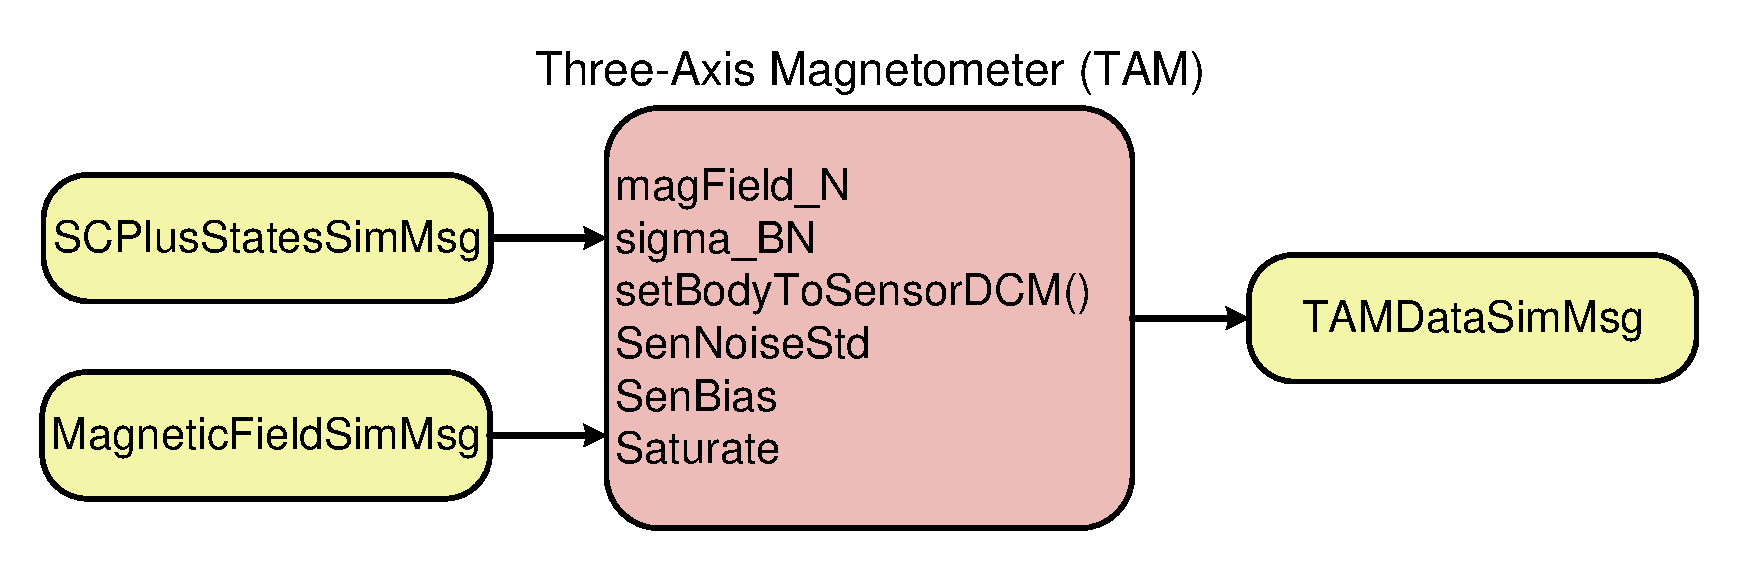
\includegraphics[width=5.5in]{Figures/moduleDiagram}
	}
	\caption{Illustration of the Magnetometer() module I/O}
	\label{fig:moduleDiagram}
\end{figure}
\subsection{General Module Behavior}
This document describes how Three-Axis Magnetometer (TAM) devices are modeled in the Basilisk software.
The purpose of this module is to implement magnetic field measurements on the sensor frame \frameDefinition{S}. 

There are a multitude of magnetic field models. As all the magnetic field models are children of {\tt MagneticFieldBase} base class, magnetometer can be created based on any of the magnetic field model. 

\subsection{Planet Centric Spacecraft Position Vector}

For the following developments, the spacecraft location relative to the planet frame is required.  Let $\bm r_{B/P}$ be the spacecraft position vector relative to the planet center.  In the simulation the spacecraft location is given relative to an inertial frame origin $O$.  The planet centric position vector is computed using
\begin{equation}
	\bm r_{B/P} = \bm r_{B/O} - \bm r_{P/O}
\end{equation}

If no planet ephemeris message is specified, then the planet position vector $\bm r_{P/O}$ is set to zero. Let $[PN]$ be the direction cosine matrix\cite{schaub} that relates the rotating planet-fixed frame relative to an inertial frame \frameDefinition{N}.  The simulation provides the spacecraft position vector in inertial frame components.  The planet centric position vector is then written in Earth-fixed frame components using
\begin{equation}
	\leftexp{P}{\bm r}_{B/P} = [PN] \ \leftexp{N}{\bm r}_{B/P}
\end{equation}




\subsection{Magnetic Field Models}
The truth of the magnetometer measurements in sensor frame coordinates with no errors are output as:
\begin{equation}
	\leftexp{S}{\bm B} = [SN] \ \leftexp{N}{\bm B}
\end{equation}
where $[SN]$ is the direction cosine matrix\cite{schaub} from $\cal{N}$ to $\cal{S}$, and $\leftexp{N}_{\bm {B}}$ is the magnetic field vector of the magnetic field model.

\subsection{Error Modeling}
The magnetic field vector of the magnetic field models is considered to be "truth" ($\ \mathbf{B}_{\mathrm{truth}} = \leftexp{S}_{\bm {B}}$). So, to simulate the errors found in real instrumentation, errors are added to the "truth" values:
\begin{equation}
\mathbf{B}_{\mathrm{measured}} = \mathbf{B}_{\mathrm{truth}} + \mathbf{e}_{\mathrm{noise}} + \mathbf{e}_{\mathrm{bias}}
\end{equation}
where $\ \mathbf{e}_{\mathrm{noise}} $ is the Gaussian noise, and $\ \mathbf{e}_{\mathrm{bias}} $ is the bias applied on the magnetic field measurements. 

\subsection{Saturation}
Sensors might have specific saturation bounds for their measurements. It also prevents the sensor for giving a value less or higher than the possible hardware output. The saturated values are:
\begin{equation}
	\mathbf{B}_{\mathrm{sat}_{\mathrm{min}}} = \mathrm{min}\big(\mathbf{B}_{\mathrm{measured}}, \mathrm{maxOutput})
\end{equation}
\begin{equation}
	\mathbf{B}_{\mathrm{sat}_{\mathrm{max}}} = \mathrm{max}\big(\mathbf{B}_{\mathrm{measured}}, \mathrm{minOutput})
\end{equation}
This is the final output of the sensor module.
